% ---------------------------------------------------
%
% Proyecto de Final de Carrera: 
% Author: Adriano dos Santos Moreira <alu0101436784@ull.edu.es>
% Chapter: Preface
% File: Cap0_Preface.tex
%
% ----------------------------------------------------

\chapter*{Preface}
\addcontentsline{toc}{chapter}{Introduction} 

High Performance Computing (HPC) \cite{Assiroj:2018:High} is a practice that utilizes powerful processors in parallel to process big data and solve complex problems at incredibly high speeds.
These systems operate at rates that are significantly faster than those of regular systems.
Supercomputers, which incorporate millions of processors, have traditionally been the norm for HPC.
Currently, the fastest supercomputer is Frontier, located in the United States, with a processing speed of 1.102 exaflops (quintillion floating point operations per second).

HPC enables organizations to gain a competitive advantage by revealing new information that advances human knowledge.
It is used for tasks such as DNA sequencing, automating stock trading, as well as running AI algorithms and simulations.
An important example regarding the latter case is autonomous driving.

All these processes analyze massive amounts of streaming data from IoT sensors, radar systems, and GPS in real time to make split-second decisions.
Higher performance in computer science is one of the key factors behind the evolution of hardware and software.
There exists a necessity for faster, more efficient calculus and data management.
The way we are able to fulfil this need has evolved with time.
For a significant number of decades, performance was increased by the upgrade in frequency of single-threaded CPUs, as seen on Figure \ref{fig:processor-trend}.
But there was a moment where an increase in frequency did not justify the also scaling power consumption.

\begin{figure}[H]
	\centering
	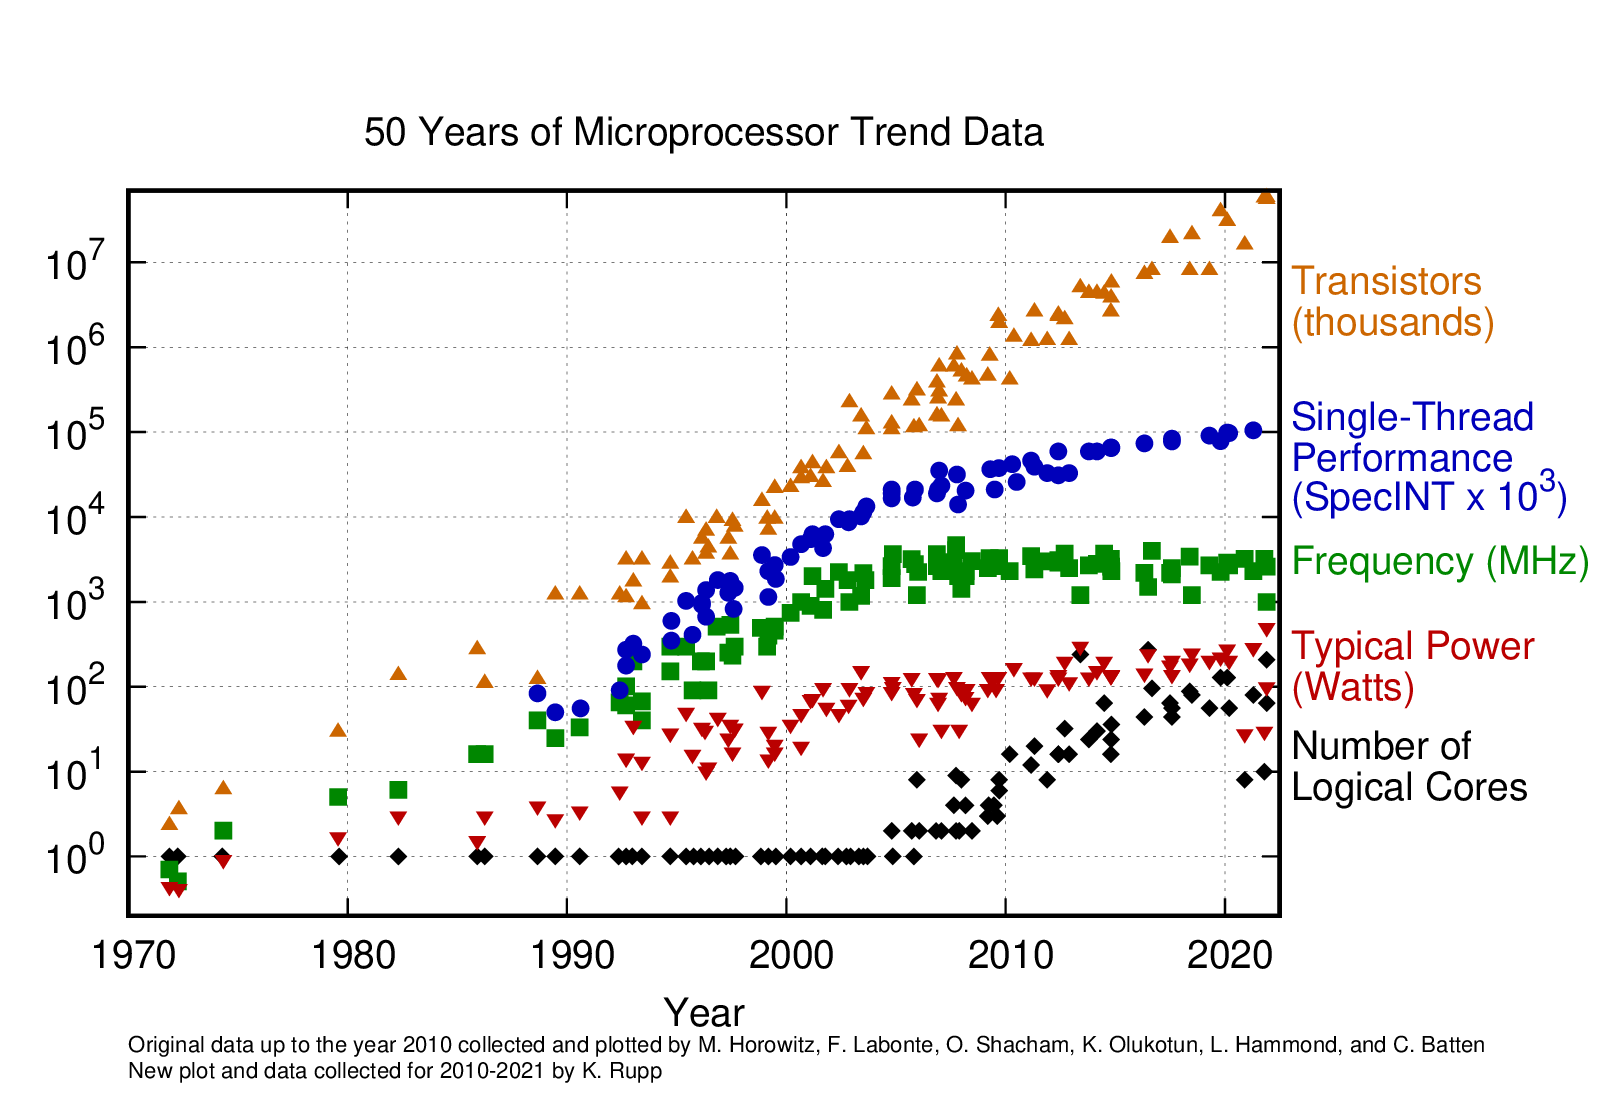
\includegraphics[width=\linewidth]{images/50-years-processor-trend.png}
	\caption{Trends of microprocessors.}
	\label{fig:processor-trend}
\end{figure}

This particular moment (around 2006) is known as ``Hit the \textit{Power Wall}'' \cite{Bose:2011:Power}.
At that time, the performance improvements of uniprocessors had come to an end due to power constraints.
This was a clear indicator that other factors have to be modified in order to gain an increase in performance. The next step is to invest on parallel architectures.

On the other hand, in the scientific and technological field, HPC is a great tool that helps researchers.
It allows the simulation of complex environments and systems (useful in physics, biology, chemistry, etc.) and the performance of intensive calculations of long duration in conventional computers, among other applications.
Due to its great time efficiency and the variety of areas of knowledge in which HPC can be used, the potential for the study of parallel computing and its application in high performance computing is clear.

There has been interest in parallel computation for a long time.
In fact, parallel computers existed before 1980 (more in-depth on page 14 of \textit{"Parallel Computing Works!"} \cite{Fox:2014:Parallel}), but greater achievements on the field were accomplished later on. Nowadays, there is a wide variety of devices for different kinds of computation objectives (CPU, FPGA, GPU, ASIC, etc.).
It has become an heterogeneous world full of distinct architectures. As a matter of fact, it has been claimed that we are currently in \textit{``A New Golden Age for Computer Architecture''} \cite{Hennessy:2019:New}.

The reasons behind the different specializations is to optimize for a particular kind of task.
This entails a more effective use of memory bandwidth and increased performance from the deliberate elimination of unnecessary accuracy, among other advantages.

With the vast amount of available devices comes the also varied collection of APIs and other utilities regarding the use of both hardware and software.
Some relevant abstraction mechanisms for parallel work include CUDA\footnote{\href{https://developer.nvidia.com/cuda-zone}{{CUDA Library of Resources} \url{https://developer.nvidia.com/cuda-zone}}}, OpenMP\footnote{\href{https://www.openmp.org}{{OpenMP API specification} \url{https://www.openmp.org}}}, OpenCL\footnote{\href{https://www.khronos.org/opencl/}{{OpenCL Main Page} \url{https://www.khronos.org/opencl/}}} and specially SYCL \cite{URL::SYCL}, but keep in mind that this is nowhere near the total amount of tools that provide this service.

This situation is quite problematic because this heterogeneous world requires heterogeneous solutions and tools.
This means that, in order to produce code that is targeted towards multiple back-ends or devices, there needs to be an abstraction that permits to do so, allowing multiple tools to work together.
Moreover, regarding HPC, both hardware and software abstraction utilities may allow for an easier way of expressing scalability, portability and versatility.
This begs for a tool that provides a more generalistic yet time and performance efficacious approach. In response to this situation comes SYCL.

% \section{SYCL overview}

SYCL is a single source, high-level, standard C++ programming model, that can target a range of heterogeneous platforms.
There are many back-end implementations that support SYCL (Fig. \ref{fig:sycl-implementations}).
We are going to focus on the Intel DPC++ branch\footnote{\href{https://github.com/intel/llvm}{{Intel oneAPI DPC++ compiler} \url{https://github.com/intel/llvm}}}.

\begin{figure}[H]
	\centering
	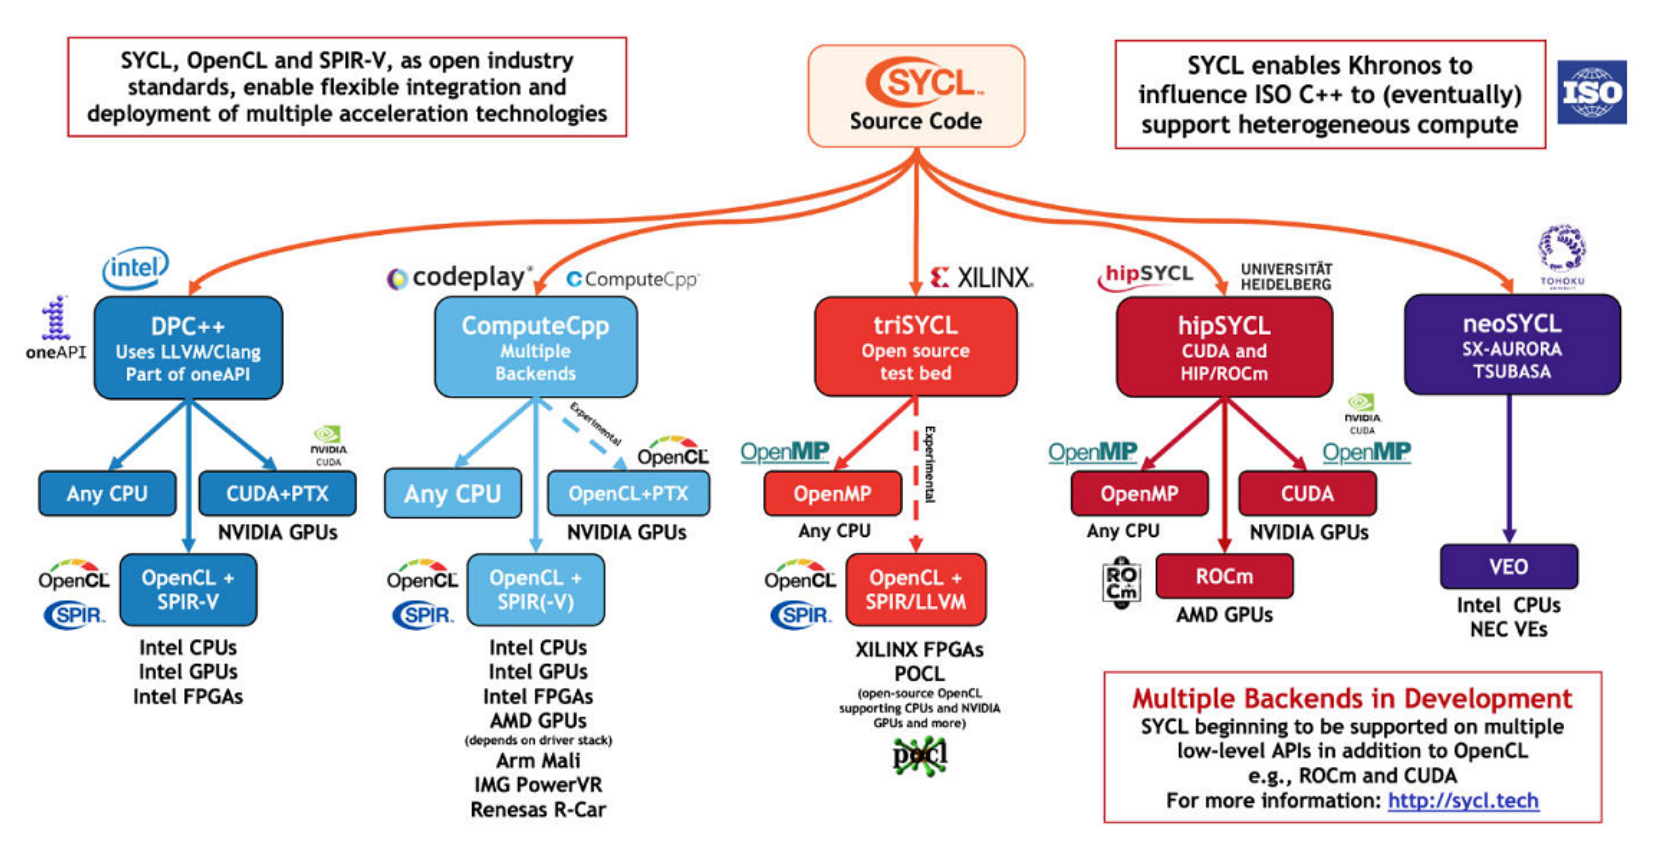
\includegraphics[width=\linewidth]{images/sycl-implementations.png}
	\caption{SYCL implementations.}
	\label{fig:sycl-implementations}
\end{figure}

This work aims to perform a deep exploration of SYCL and its capabilities, as well as producing benchmark tests with other platforms such as CUDA.
Another topic of interest is the analysis and implementation of different data management models.
As a given, this study will be covering these tasks from a HPC perspective when possible.

All the code examples written by the student for this work follow the principles of Martin's Clean Code book \cite{Martin:2009:Clean} and conform to the Google's Style Guide\footnote{\href{https://google.github.io/styleguide/}{{Google Style Guides} \url{https://google.github.io/styleguide/}}}, while code excerpts from other works will remain essentially untouched.
The reason behind the decision to write code using Google's Style is completely arbitrary, the importance of choosing a style relies on being consistent with its use: \textit{``The last thing we want to do is add more complexity to the source code by writing it in a jumble of different individual styles.'' - Robert C. Martin}.

Every piece of code written by the student for this project is publicly available on the GitHub repository dedicated to this work \cite{URL::TFG}.
Also note that every listing has a link to its original source and in the case of the student's code, there will be a direct link to the corresponding file in the work's repository, labeled as \textit{``See on GitHub''}.
